% *==================================================================================*
% *                     Review vs. Camera-Ready settings                             *
% *==================================================================================*
%
% REVIEW: Use the following command for submitting the paper (double-blind,
% for review):
% \documentclass{Interspeech}
%
% CAMERA-READY: Use the following command for the camera-ready version, one
% affiliation per line:
\documentclass[cameraready]{Interspeech}
\usepackage{amsmath}
\usepackage{amssymb}
\usepackage{hyperref}
\usepackage{xurl}
\hypersetup{
    colorlinks=true, % Colours links instead of ugly boxes
    urlcolor=blue,   % Colour for external hyperlinks
    linkcolor=blue,  % Colour of internal links
    citecolor=red    % Colour of citations
}
\usepackage{enumitem}
\usepackage{graphicx}
% *==================================================================================*


% **************************************
% *                                    *
% *      STOP !   DO NOT DELETE !      *
% *          READ THIS FIRST           *
% *                                    *
% * This template also includes        *
% * important INSTRUCTIONS that you    *
% * must follow when preparing your    *
% * paper. Read it BEFORE replacing    *
% * the content with your own work.    *
% **************************************

%==================================================================================
% Title
% Must exactly match the title entered into the paper submission system
\title{Design and Evaluation of Face Recognition Systems Under Adversarial Attacks}

%==================================================================================
% Authors
% The order of authors here must exactly match the order entered into the paper submission system
% Note that the COMPLETE list of authors MUST be entered into the paper submission system at the outset, including when submitting your manuscript for double-blind review
% The ORCID number is still optional but will become mandatory in the future years. It is strongly encouraged to get an ORCID for each cu-author.
% Middle names, including initials, must be included in the first name
\author[affiliation={1}]{Maria Teresa}{Franco}
\author[affiliation={1}]{Luqi}{Sun}
\author[affiliation={1}]{MaKhaila}{Bentil}
\author[affiliation={1}]{YiChiao}{Wang}
\author[affiliation={1}]{Xiutian}{Zhao}



% The maximum number of authors in the author list is 20. If the number of contributing authors is more than this, they should be listed in a footnote or the acknowledgement section.

%==================================================================================
% Affiliations

\address{
$^1$ Johns Hopkins University\\
{\small \texttt{
mfranc39@jh.edu (mfranc39),
lsun59@jh.edu (lsun59),
mbentil1@jh.edu (mbentil1),
ywan1149@jh.edu (ywan1149),
xzhao117@jh.edu (xzhao117)
}}
}


%==================================================================================
% Emails
\email{}

%==================================================================================
% Keywords
\keywords{Face Recognition, Attack}

\newcommand{\blue}[1]{\textcolor{blue}{#1}}
\newcommand{\red}[1]{\textcolor{red}{#1}}
\usepackage{comment}

%==================================================================================
% Content

\begin{document}

\maketitle

% the abstract here must exactly match the abstract entered into the paper submission system

\section{Motivation}
Identity verification is an important branch of cybersecurity. Utilizing biometric measurements, such as face, fingerprint, iris, and voice, for authentication purposes has attracted widespread attention over the past two decades due to its good usability and high reliability. Among them, face verification (Face ID) has become one of the most widely used biometric authentication technologies due to its contactless and user-friendly nature~\cite{jha2022face}. However, with the widespread deployment of Face ID systems, they have been continuously subjected to various adversarial example attacks, seriously threatening the security and reliability of the systems~\cite{Sharif2016}. Therefore, enhancing their resistance to attacks is of significant research importance.

Against this backdrop, the goal of this project is to set up a Face ID system and study which adversarial attacks it is most vulnerable to.
We aim to improve the security of the Face ID system and anticipate possible attacks.
% , including deepfake-based impersonation.  
We will also explore retraining the model with adversarial examples and evaluate how this affects robustness against these attacks. We hypothesize that adversarial training improves robustness under attack.

% Modern Face ID systems are widely used for authentication (phones, banking, access control), but they are not designed to be robust by default against adversarial threats. 
% The thesis behind this is that a face recognition system trained for standard accuracy is highly vulnerable to adversarial and synthetic impersonation attacks, but adversarial training significantly improves robustness.

% Therefore our project has to main objectives: 
%     \begin{itemize}
%         \item Build a baseline Face ID system.
%         \item Test it against several digital adversarial attacks and harden it. % as we don't cover physical ones (e.g., printed face, screen display)
%     \end{itemize}

\vspace{-3mm}
\section{Dataset and Task}
Our first objective is to build a Face ID (face verification) system, which requires identity labels and multiple images per identity, rather than attribute classification (gender, race, age). We plan to use the publicly available CASIA-WebFace dataset~\cite{CASIA}, which contains approximately 10,575 identities and 494,414 face images collected from the Internet. The data are organized in the form of “one folder per person, multiple images per identity.” This dataset covers a wide range of variations in pose, expression, illumination, and resolution, effectively reflecting the complexity of faces in real-world scenarios.





\vspace{-2mm}
\section{Architecture}

\subsection{Face ID system}
There are two possible options to proceed:
\begin{enumerate}[label=\Roman*)]
    \item  Use an \href{https://medium.com/@ichigo.v.gen12/arcface-architecture-and-practical-example-how-to-calculate-the-face-similarity-between-images-183896a35957#a5a8}{ArcFace}~\cite{ArcFace} embedding model as a feature extractor (using the library \href{https://pypi.org/project/insightface/}{InsightFace}), design the verification logic and focus on implementing adversarial attacks and adversarial training.
    \item  Build the model and train it from scratch using Convolutional Neural Networks (CNN) like the ResNet-18 architecture ~\cite{ResNet} to enable training on our laptops. Design the verification logic and then focus on implementing adversarial attacks and adversarial training.
\end{enumerate}

\vspace{-1mm}
\subsection{Adversarial Attacks}
We plan to focus on digital adversarial example attacks~\cite{GoodfellowAdversarial} and experiment with two white-box attacks and one black-box attack. We evaluate both impersonation (FAR) and dodging (FRR) under the verification setting:

\begin{enumerate}[label=\Roman*)]
    \item Projected Gradient Descent (PGD): an iterative extension of FGSM and a strong white-box attack against neural networks.
    \item Carlini-Wagner (CW): a strong optimization-based attack for targeted objectives in verification (e.g., impersonation or dodging).
    \item Transfer attack: craft adversarial examples using a surrogate model and test their transferability to the target model.
\end{enumerate}

\section{Experimental Plan and Deliverables}
\begin{enumerate}[label=\Roman*)]
    \item Implement baseline verification pipeline with calibrated thresholds. 
    \item Establish clean benchmark performance on verification pairs from a held-out split; calibrate the decision threshold on a validation set and report FAR, FRR, and EER.
    \item Implement attacks (white-box PGD/CW and transfer) and report attack success rates and robust verification metrics.
    \item Implement adversarial training and re-evaluate (clean + robust metrics).
\end{enumerate}

\section{Experiment}

\subsection{Baseline results (ArcFace / InsightFace) on LFW eval bin}

\begin{table}[htb!]
\centering
\resizebox{\columnwidth}{!}{%
\begin{tabular}{lrrrrrr}
\toprule
Dataset & \#Pairs & \#Same & \#Diff & EER $\downarrow$ & FAR@$\tau_{\text{EER}}$ $\downarrow$ & FRR@$\tau_{\text{EER}}$ $\downarrow$ \\
\midrule
LFW (eval \texttt{.bin}) & 6000 & 3000 & 3000 & 0.0035 & 0.0040 & 0.0030 \\
\bottomrule
\end{tabular}%
}
\vspace{2mm}
\caption{Clean face verification baseline using an ArcFace-style embedding model (InsightFace \texttt{buffalo\_l} recognition backbone \texttt{w600k\_r50}). Verification is performed by cosine similarity with threshold $\tau$. We report the equal error rate (EER) and FAR/FRR at the EER-selected threshold.}
\label{tab:lfw_baseline}
\end{table}

\subsubsection{Baseline evaluation protocol.}
We evaluate face verification on the InsightFace-formatted \footnote{\url{https://pypi.org/project/insightface/}} LFW benchmark stored as a binary pair file
\texttt{~/casia-webface/eval/lfw.bin} \footnote{\url{https://www.kaggle.com/datasets/debarghamitraroy/casia-webface}}.
This file contains a tuple $(\texttt{bins}, \texttt{issame})$ loaded via Python pickle, where
\texttt{bins} is a list of encoded face images (bytes) and \texttt{issame} is a boolean list indicating whether each pair is from the same identity.
Pairs are indexed deterministically: for pair index $i\in\{0,\dots,5999\}$, the two images are \texttt{bins[2*i]} and \texttt{bins[2*i+1]}, with label \texttt{issame[i]} (1 for same-identity, 0 otherwise).
No images are excluded in our run (\texttt{detect\_or\_decode\_fail}=0).

\subsubsection{Model and preprocessing.}
We use the InsightFace \texttt{buffalo\_l} model package and the recognition backbone \texttt{w600k\_r50.onnx} (512-D embeddings).
For each image, we decode bytes using OpenCV (\texttt{cv2.imdecode}) to a BGR array and apply a fixed resize to $112\times112$.
We use a \emph{recognition-only} pipeline (no face detection/alignment), extract embeddings with \texttt{get\_feat}, and compute cosine similarity between the two embeddings in a pair.
A pair is accepted as a match if similarity $\ge \tau$.

\subsubsection{Results and interpretation.}
On all 6000 LFW pairs (3000 same, 3000 different), the ArcFace baseline achieves an EER of 0.0035.
At the threshold selected from the ROC point closest to FAR$=$FRR ($\tau_{\text{EER}}=0.1767$), we obtain FAR$=0.0040$ and FRR$=0.0030$.
Concretely, this corresponds to approximately $0.0040\times 3000\approx 12$ false accepts among impostor pairs and $0.0030\times 3000\approx 9$ false rejects among genuine pairs.
These results indicate strong clean verification performance and provide a stable baseline for evaluating adversarial attacks.

\vspace{-2mm}
\subsection{One Pixel Attack}
\emph{To be added.}

\subsection{PGD Attack}
\emph{To be added.}

\subsection{Carlini-Wagner (C\&W) Attack Implementation}
Adversarial attacks on face recognition systems have been demonstrated in prior work~\cite{Sharif2016}. We implement the Carlini-Wagner (C\&W) optimization-based attack~\cite{Zachariah2023CW}, adapted from image classification to face verification.

\subsubsection{Formulation and verification adaptation.}
Given an original image $\mathbf{x} \in [0,1]^{C \times H \times W}$ and a face recognition model $\phi$ producing embeddings $\phi(\mathbf{x}) \in \mathbb{R}^d$, the C\&W attack seeks a perturbed image $\mathbf{x}'$ that minimizes the $\ell_2$ perturbation while achieving the attack objective~\cite{ArcFace}:
\begin{equation}
\min_{\mathbf{x}'} \; \lVert \mathbf{x}' - \mathbf{x} \rVert_2^2 + c \cdot f(\mathbf{x}')
\end{equation}
where $f$ encodes the attack goal. We use the tanh parameterization to keep pixels in $[0,1]$:
\begin{equation}
\mathbf{x}' = \tfrac{1}{2}\bigl(\tanh(\mathbf{w}) + 1\bigr)
\end{equation}
We optimize over $\mathbf{w}$ with Adam and perform binary search over $c$. For \textbf{Impersonation (FAR)}, we require
\begin{equation}
\cos\bigl(\phi(\mathbf{x}'), \mathbf{e}_t\bigr) > \cos\bigl(\phi(\mathbf{x}'), \mathbf{e}_s\bigr)
\end{equation}
so the adversarial verifies as the target identity $\mathbf{e}_t$; for \textbf{Dodging (FRR)}, we minimize $\cos(\phi(\mathbf{x}'), \mathbf{e}_s)$ so the face is no longer verified as the source $\mathbf{e}_s$. The loss $f$ uses hinge-style objectives over these cosine similarities.

\subsubsection{Experimental setup.}
The attack integrates with our ArcFace baseline (InsightFace \texttt{w600k\_r50}) via a PyTorch wrapper. We run impersonation and dodging via \texttt{run\_cw\_attack.py} on CASIA-WebFace extracted face pairs. Unit tests validate both modes on linear placeholder models and on real CASIA images using the ArcFace/ONNX backbone.

\subsubsection{Results.}
Unit tests (4 tests: impersonation and dodging on linear models, plus impersonation and dodging on real CASIA images) pass in approximately 2 minutes. Runs via \texttt{run\_cw\_attack.py} use one (source, target) pair per run (batch=1), with 1000 optimizer steps per $c$ value and 7 binary search steps over $c$ (7000 gradient steps total). On CPU, a full impersonation run takes approximately 3--4 hours; on GPU it would complete in minutes. For a representative CASIA pair (source: identity 0000045, target: identity 0000099), we obtain perturbation $\boldsymbol{\delta} = \mathbf{x}' - \mathbf{x}$ with $\lVert \boldsymbol{\delta} \rVert_2 = 2.25$. The adversarial image is visually nearly indistinguishable from the source while causing the model to verify it as the target identity. Our ArcFace baseline uses threshold $\tau_{\text{EER}} \approx 0.18$ for same-identity verification on LFW; the C\&W attack achieves Eq.\,(3), as validated by unit tests and the successful impersonation output.

\begin{figure}[htb]
\centering
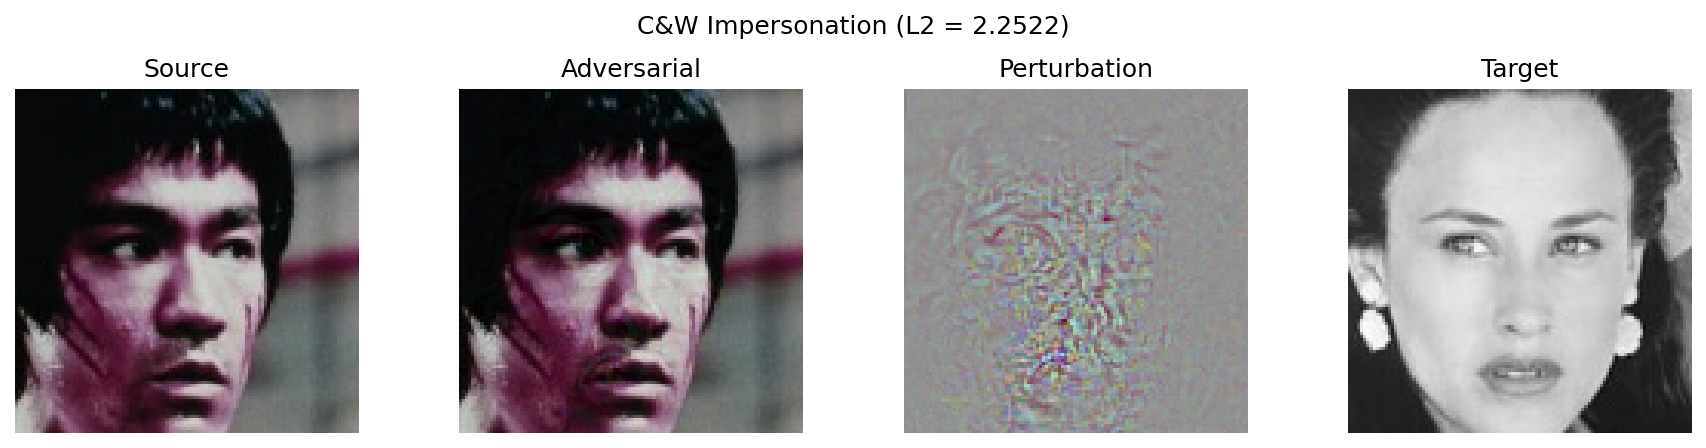
\includegraphics[width=\linewidth]{figures/cw_impersonation.png}
\caption{C\&W impersonation: source $\mathbf{x}$, adversarial $\mathbf{x}'$, perturbation $\boldsymbol{\delta} = \mathbf{x}' - \mathbf{x}$ (scaled for visibility), and target $\mathbf{x}_{\text{tgt}}$. $\lVert \boldsymbol{\delta} \rVert_2 = 2.25$. The adversarial verifies as the target identity under ArcFace.}
\label{fig:cw_impersonation}
\end{figure}

\bibliographystyle{IEEEtran}
\nocite{*}
\bibliography{mybib}

\end{document}

%%% Local Variables:
%%% mode: LaTeX
%%% TeX-master: t
%%% End:
